\chapter{LANDASAN TEORI}
\section{Tinjauan Pustaka}
Dalam penelitian ini, beberapa referensi kepustakaan yang bersumber pada penelitian sebelumnya diambil sebagai bahan referensi. Referensi ini digunakan untuk membantu dalam menyelesaikan penelitian yang sedang dilakukan. Peneliti menggunakan referensi-referensi tersebut sebagai acuan dan sumber informasi untuk memperdalam pemahaman tentang topik yang sedang diteliti.

Pada penelitian terdahulu \textcite{suryadibrata2020visualisasi} membuat visualisasi algoritma \textit{K-Means Clustering} dalam bentuk 3D menggunakan unity dan menggunakan bahasa pemrograman C\char"0023\ yang dikembangkan dalam model \textit{Waterfall}. Aplikasi visualisasi ini bertujuan untuk membantu pelajar dalam memahami algoritma \textit{K-Means Clustering}. Aplikasi dalam penelitian ini mengimplementasikan animasi dari proses perhitungan jarak antara setiap vektor data dan setiap vektor pusat yang ada menggunakan sebuah garis pembantu. Dalam proses visualisasi garis pembantu berperan untuk menunjukkan proses pencarian jarak terdekat dari setiap vektor data.

Penelitian kedua yang dilakukan oleh \textcite{zarkasyi2015pengembangan} menggunakan aplikasi GeoGebra untuk media pembelajaran dengan tujuan memvisualisasikan penggunaan integral pada siswa SMA. Adapun kriteria kualitas media pembelajaran yang meliputi aspek kualitas visual dan kualitas teknis. Dengan menggunakan media pembelajaran tersebut, diharapkan dapat meningkatkan pemahaman siswa mengenai penggunaan integral. Metode yang digunakan dalam penelitian ini menggunakan model pengembangan ADDIE (\textit{Analysis, Design, Development, Implementation, Evaluation}). Menurutnya seorang guru harus menciptakan pembelajaran yang dapat membantu siswa membayangkan atau memvisualisasikan dengan mengembangkan media pembelajaran. Dia menekankan bahwa media pembelajaran dapat menjadi perantara yang membantu siswa mengurangi keabstrakan objek matematika yang sulit dipahami.

Dengan menggunakan media interaktif, pengajar dapat lebih mudah dalam proses pengajaran dan mahasiswa dapat lebih tertarik dan termotivasi untuk menumbuhkan rasa keingintahuannya, karena materi yang disampaikan dapat disertai dengan tampilan multimedia interaktif \cite{maulana2021penerapan}.

Berdasarkan tinjauan pustaka yang telah disajikan, dapat disimpulkan bahwa penggunaan aplikasi visualisasi dan media pembelajaran interaktif dapat meningkatkan kualitas pembelajaran serta motivasi belajar mahasiswa. Penelitian terdahulu yang telah dilakukan oleh para peneliti sebelumnya dapat menjadi acuan dan bahan pertimbangan dalam menganalisis hasil penelitian ini. Diharapkan penelitian ini dapat memberikan sumbangsih bagi pengembangan media pembelajaran yang lebih inovatif dan efektif untuk meningkatkan kualitas pendidikan.

Penelitian ini memiliki kesamaan dengan penelitian sebelumnya yaitu keduanya menggunakan aplikasi visualisasi sebagai media pembelajaran. Namun, terdapat perbedaan dimana penelitian sebelumnya memvisualisasikan K-Means Clustering dengan menggunakan bahasa pemrograman C\char"0023\ berbasis aplikasi \textit{desktop}, sedangkan penelitian ini memvisualisasikan operasi pengolahan citra digital dengan menggunakan bahasa pemrograman \textit{JavaScript} berbasis \textit{Web}.
\section{Dasar Teori}
\subsection{Pengolahan Citra Digital}
\textcite{munantri2020aplikasi} menjelaskan bahwa citra digital adalah gambar dua dimensi yang dihasilkan dari proses sampling pada gambar analog dua dimensi yang kontinu, sehingga menjadi gambar diskrit yang dapat diolah oleh komputer. Citra digital disimpan dalam bentuk data numerik yang menunjukkan besar intensitas pada masing-masing pikselnya. Oleh karena itu, citra digital dapat diolah dengan menggunakan komputer untuk berbagai keperluan seperti pengolahan gambar, analisis citra, dan pengenalan pola.

Masih menurut \textcite{munantri2020aplikasi} menjelaskan bahwa pengolahan citra digital merupakan ilmu yang mempelajari berbagai hal terkait dengan perbaikan kualitas gambar, transformasi gambar, pemilihan citra ciri yang optimal, penyimpanan data, transmisi data, dan waktu proses data. Proses pengolahan citra dapat dijelaskan dengan menggunakan diagram sederhana yang meliputi beberapa tahap, seperti perbaikan kualitas citra, transformasi citra, pemilihan citra ciri, reduksi dan kompresi data, transmisi data, dan waktu proses data. Dalam pengolahan citra digital, teknik-teknik pengolahan yang digunakan dapat berbeda-beda tergantung pada jenis citra dan tujuan analisis yang ingin dicapai.

Dari uraian diatas penulis menyimpulkan bahwa citra digital adalah hasil dari proses sampling pada gambar analog dua dimensi yang kemudian diubah menjadi gambar diskrit dengan data numerik yang merepresentasikan besar intensitas pada masing-masing piksel. Citra digital dapat diolah dengan menggunakan komputer dan teknik-teknik pengolahan citra yang berbeda-beda tergantung pada jenis citra dan tujuan analisis yang ingin dicapai. Proses pengolahan citra digital meliputi berbagai tahap seperti perbaikan kualitas citra, transformasi citra, pemilihan citra ciri, reduksi dan kompresi data, transmisi data, dan waktu proses data. Dalam ilmu pengolahan citra digital, terdapat berbagai macam teknik yang dapat digunakan untuk mengambil informasi dari citra digital atau memperbaiki kualitas citra.

\subsection{Segmentasi}

Menurut \textcite{IPI1759345} menjelaskan bahwa tepi atau edge pada pengolahan citra digital merujuk pada perubahan mendadak nilai intensitas derajat keabuan dalam jarak yang dekat. Sebuah titik dapat dikategorikan sebagai tepi ketika memperlihatkan perbedaan nilai piksel yang signifikan dengan nilai piksel tetangganya. Untuk mendeteksi tepi dalam citra digital, diperlukan operasi \textit{edge detection} guna mengenali garis tepi yang membatasi wilayah citra homogen yang memiliki perbedaan tingkat kecerahan. Dalam bidang pengolahan citra, deteksi tepi menjadi hal yang penting karena berperan dalam menghasilkan tepi-tepi pada obyek citra digital.Beberapa teknik untuk mendeteksi tepi:

\begin{enumerate}[leftmargin=1cm, itemindent=0.6cm,labelwidth=15pt, labelsep=5pt, listparindent=1cm,align=left]

    \item Operator \textit{Roberts}

    Operator Roberts adalah operator yang berbasis gradien yang menggunakan dua buah kernel yang berukuran 2x2 piksel. Operator ini mengambil arah diagonal untuk penentuan arah dalam penghitungan nilai gradien, sehingga sering disebut dengan operator silang \textcite{mulyanto2009teori}.

\begin{figure*}[ht]
    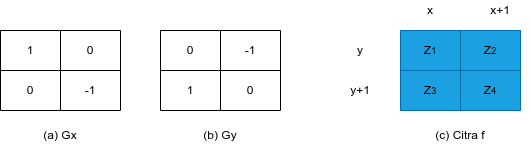
\includegraphics[width=0.85\textwidth, center]{images/Robert.png}
    \caption{Operator Robert}
\end{figure*}

    Bentuk dari operator \textit{roberts} ditunjukkan pada gambar 2.1. Misal f adalah citra yang akan dikenai operator \textit{roberts}. Maka, nilai operator Robert pada (y, x) didefinisikan sebagai

\begin{equation}
r(y,x) = \sqrt{(z_1 - z_4)^2 + (z_3 - z_2)^2}
\end{equation}

Dalam hal ini, z1 = f(y,x), z2 = f(y,x+1), z3 = f(y+1,x), dan z4 = f(y+1,x+1).

\item Operator \textit{Prewitt}

\begin{figure*}[ht]
    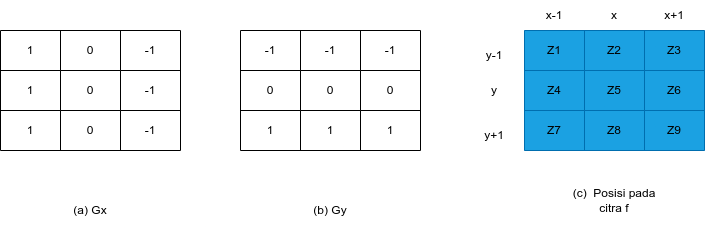
\includegraphics[width=0.85\textwidth, center]{images/Prewitt.png}
    \caption{Operator Prewitt}
\end{figure*}

    Metode \textit{Prewitt} merupakan pengembangan dari metode Robert yang ditemukan oleh Prewitt pada tahun 1966. Metode \textit{Prewitt} menggunakan filter HPF (\textit{High Pass Filter}) yang diberi satu angka nol penyangga. Metode ini mengambil prinsip dari fungsi laplacian sebagai fungsi untuk membangkitkan HPF (\textit{High Pass Filter}). Kernel filter yang digunakan dalam metode Prewitt ini bisa dilihat pada gambar 2.2.

    Bentuk dari operator \textit{prewitt} ditunjukkan pada gambar 2.2. Misal f adalah citra yang akan dikenai operator \textit{prewitt}. Maka, nilai operator prewitt pada (y, x) didefinisikan sebagai

\begin{equation}
r(y,x) =
\sqrt{
\begin{aligned}
(f(y-1,x-1)+f(y,x-1)+f(y+1,x-1)\\
-f(y-1,x+1)-f(y,x+1)-f(y+1,x+1))^2\\
+(f(y+1,x-1)+f(y+1,x)+f(y+1,x+1)\\
-f(y-1,x-1)-f(y-1,x)-f(y-1,x+1))^2
\end{aligned}
}
\end{equation}

    \item Operator \textit{Sobel}

    Operator \textit{sobel} adalah operator yang banyak digunakan sebagai pendeteksian tepi karena kesederhanaannya. Operator \textit{sobel} merupakan pengembangan dari operator \textit{robert} yang diberi satu angka nol penyangga. Berbeda dengan operator \textit{prewitt} yang lebih sensitif terhadap tepi vertikal dan horizontal, operator \textit{sobel} lebih sensitif terdapap tepi diagonal. Kelebihan dari metode \textit{sobel} ini adalah kemampuan untuk mengurangi \textit{noise} sebelum melakukan perhitungan pendeteksian tepi.

\begin{figure*}[ht]
    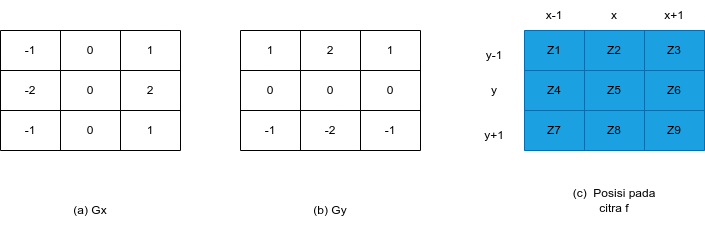
\includegraphics[width=0.85\textwidth, center]{images/Sobel.png}
    \caption{Operator Sobel}
\end{figure*}

Operator sobel adalah magnitude dari gradien yang dihitung dengan

\begin{equation}
M =
\sqrt{
\begin{aligned}
S_x^2+S_y^2
\end{aligned}
}
\end{equation}

Keterangan

M = Besar gradien operator sobel

Sx = Gradien \textit{sobel} arah horizontal

Sy = Gradien \textit{sobel} arah vertikal

    \item Operator \textit{Laplacian}

    Operator Laplacian merupakan operator turunan kedua yang bersifat omnidirectional, yakni menebalkan bagian tepi ke segala arah. Namun, operator Laplacian memiliki kelemahan yakni peka terhadap derau, memberikan ketebalan ganda dan tidak mampu mendeksi arah tepi \cite{kadir2013pengolahan}.

\begin{figure*}[ht]
    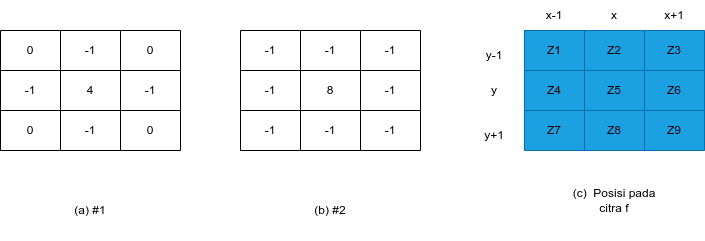
\includegraphics[width=0.85\textwidth, center]{images/Laplacian.png}
    \caption{Operator Laplacian}
\end{figure*}


    Berdasarkan cadar \#1 pada gambar 2.4(a), nilai operator Laplacian pada (y,x) didefinisikan sebagai

\begin{equation}
l(y,x) =
\begin{aligned}
4f(y,x)-[f(y-1,x)+f(y,x-1)+f(y,x+1)+f(y+1,x)]
\end{aligned}
\end{equation}

    \item Operator \textit{Canny}

    Operator Canny ditemukan oleh John Canny pada tahun 1986 yang terkenal sebagai operator deteksi tepi yang optimal. Algoritma ini memberikan tingkat kesalahan yang rendah. Terdapat enam langkah yang dilakukan untuk mengimplementasikan deteksi tepi Canny. Langkah tersebut dijabarkan sebagai berikut

\begin{figure*}[ht]
    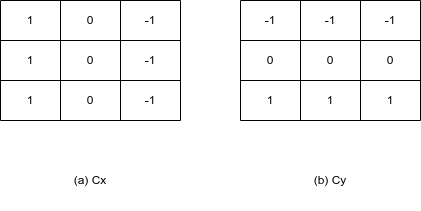
\includegraphics[width=0.85\textwidth, center]{images/Canny.png}
    \caption{Operator Canny}
\end{figure*}

    \begin{enumerate}
        \item Langkah 1

        Pertama dilakukan penapisan terhadap citra dengan tujuan untuk menghilangkan derau menggunakan filter Gaussian dengan kadar sederhana dengan ketentuan kadar yang digunakan berukuran jauh lebih kecil dari pada ukuran citra.

        \item Langkah 2

        Setelah penghalus gambar terhadap derau dilakukan, selanjutnya proses mendapatkan kekutan tepi (edge strenght) dengan menggunakan operator Gaussian. Gradien citra dapat dihitung dengan rumus

        \begin{equation}
        \left | G \right | = \left | Gx \right | + \left | Gy \right |
        \end{equation}

        \item Langkah 3

        Menghitung arah tepi. Rumus yang digunakan adalah

        \begin{equation}
        theta= \tan ^{-1}(GxGy)
        \end{equation}

        \item Langkah 4

        Menghubungkan arah tepi dengan sebuah arah yang dapat dilacak citra.

    \item Langkah 5

        Proses hysteresis, proses ini menghilangkan garis-garis yang terputus.
    \end{enumerate}

\end{enumerate}

\subsection{Media Pembelajaran}
Menurut \textcite{arsyad2015media} kata media berasal dari bahasa latin \textit{medius} yang secara harfiah berarti ``tengah'', ``perantara'' atau ``pengantar'', yang dalam bahasa arab diartikan sebagai perantara atau pengantar pesan dari pengirim kepada penerima pesan. Oleh karena itu, media diartikan sebagai alat yang menyampaikan atau mengantarkan pesan-pesan pengajaran.

\textcite{nurrita2018pengembangan} menjelaskan bahwa media pembelajaran berperan sebagai alat yang dapat membantu proses belajar mengajar sehingga makna pesan yang disampaikan dapat menjadi lebih jelas dan tujuan pendidikan atau pembelajaran dapat tercapai dengan efektif dan efisien.

Berdasarkan uraian diatas dapat disimpulkan bahwa media pembelajaran merupakan alat atau sarana yang berperan sebagai perantara atau pengantar pesan dalam proses belajar mengajar. Dalam proses pembelajaran, media pembelajaran dapat membantu membuat pesan yang disampaikan menjadi lebih jelas dan tujuan pembelajaran dapat tercapai dengan efektif dan efisien. Oleh karena itu, penggunaan media pembelajaran sangat penting dalam proses belajar mengajar untuk mencapai hasil yang optimal.

\subsection{Visualisasi}
Visualisasi memiliki beberapa landasan teori yang mendasar, di antaranya adalah teori pengolahan informasi, teori persepsi visual, dan teori kognitif. Teori pengolahan informasi menjelaskan bahwa manusia memproses informasi dengan cara menerima, menyimpan, mengorganisir, dan mengambil kembali informasi dalam memori. Teori ini menjadi dasar bagi visualisasi karena visualisasi digunakan untuk mempermudah pengolahan informasi dengan menggambarkan data dalam bentuk visual yang mudah dipahami.

Teori persepsi visual menjelaskan tentang bagaimana manusia mengamati dan menginterpretasikan dunia visual. Teori ini menjelaskan bagaimana manusia memahami bentuk, warna, ukuran, dan posisi objek dalam lingkungan visual. Teori ini menjadi penting dalam visualisasi karena visualisasi berupaya untuk membuat gambaran yang tepat dan mudah dipahami oleh pengamat.

Sedangkan teori kognitif membahas tentang bagaimana manusia memproses, menyimpan, mengambil, dan menggunakan informasi yang telah dipelajari. Teori ini menjadi dasar bagi pengembangan visualisasi karena visualisasi bertujuan untuk meningkatkan pemahaman dan retensi informasi pada manusia dengan menyajikan informasi dalam bentuk yang mudah diingat dan dipahami.

Dari ketiga landasan teori di atas, dapat disimpulkan bahwa visualisasi sebagai alat bantu memahami informasi berusaha mempermudah pengolahan informasi manusia dengan menggunakan teori pengolahan informasi, teori persepsi visual, dan teori kognitif sebagai dasar pengembangan.

\subsection{Web}
Web atau \textit{World Wide Web} (WWW) adalah sistem informasi global yang terhubung melalui jaringan internet dan digunakan untuk mengakses dan berbagi informasi di seluruh dunia. Web pertama kali diperkenalkan pada tahun 1989 oleh Tim Berners-Lee, seorang ilmuwan komputer dari Inggris. Dalam pengertian umum, web adalah kumpulan dokumen atau halaman web yang terdiri dari teks, gambar, video, dan berbagai jenis konten multimedia lainnya.

Pada awalnya, web hanya digunakan sebagai alat untuk membagikan informasi dan sebagai tempat untuk mengakses situs web. Namun, seiring dengan perkembangan teknologi, web kini telah menjadi lebih interaktif dan dinamis. Contohnya adalah adanya aplikasi web yang memungkinkan pengguna untuk melakukan transaksi online, berinteraksi dengan orang lain, bermain game, bahkan menjadi media pembelajaran.

Web sendiri terdiri dari tiga komponen utama, yaitu bahasa markup (HTML), style sheet language (CSS), dan bahasa scripting (JavaScript). HTML digunakan untuk membuat struktur dasar halaman web, sedangkan CSS digunakan untuk mendesain tampilan halaman web, dan JavaScript digunakan untuk membuat halaman web menjadi interaktif.

\subsection{Alat Bantu Pengembangan di Perancangan Sistem}

\begin{enumerate}[leftmargin=1cm, itemindent=0.6cm,labelwidth=15pt, labelsep=5pt, listparindent=1cm,align=left]

    \item DFD (Data \textit{Flow Diagaram})

    Dalam perancangan sistem, DFD (Data Flow Diagram) dianggap sebagai sarana yang penting untuk memberikan gambaran logika secara independen terhadap perangkat lunak, perangkat keras, struktur data, atau organisasi file. Hal ini dapat dilihat dari penggunaan DFD dalam beberapa bentuk seperti diagram konteks dan diagram level n, yang digunakan untuk menggambarkan suatu sistem dengan lebih terstruktur dan sistematis \textcite{khotijah2016perancangan}.

    DFD terdiri dari dua jenis diagram, yaitu diagram konteks dan diagram level n. Diagram konteks digunakan untuk menggambarkan hubungan sistem dengan entitas luar yang terkait, serta aliran data yang masuk dan keluar dari sistem. Sedangkan diagram level n digunakan untuk menggambarkan detail lebih lanjut dari diagram konteks, dengan memperlihatkan proses-proses, data yang digunakan dan dihasilkan, serta interaksi antara sistem dengan entitas luar.

    Keuntungan dari penggunaan DFD adalah memudahkan dalam mengidentifikasi kebutuhan fungsional suatu sistem, mengidentifikasi kekurangan dan kelebihan sistem yang ada, serta memberikan gambaran tentang cara sistem harus dirancang dan diimplementasikan. DFD juga membantu dalam mengkomunikasikan gagasan antara para analis dan pemangku kepentingan terkait sistem yang akan dibangun.

    \item Flowchart

    menyatakan bahwa desain arsitektur program memiliki peran penting dalam menentukan hubungan antara elemen-elemen struktural utama dalam program. Desain arsitektur dapat dijabarkan dalam bentuk diagram alir program atau flowchart, yang menggunakan simbol-simbol khusus untuk menyatakan aliran proses program dan alur proses yang dikehendaki.

    Diagram alir program terdiri dari beberapa simbol yang masing-masing memiliki arti dan fungsi yang berbeda-beda. Beberapa simbol umum yang sering digunakan dalam flowchart antara lain:

    \begin{enumerate}
        \item Oval: Menunjukkan awal atau akhir dari proses.
        \item Kotak: Menunjukkan proses yang harus dilakukan
        \item Panah: Menunjukkan arah aliran proses
        \item Diamond: Menunjukkan kondisi atau percabangan dalam proses
    \end{enumerate}

    Dalam membuat flowchart, perlu diperhatikan juga urutan proses yang logis dan jelas, sehingga dapat memudahkan penggunaan flowchart dalam memahami alur proses program. Selain itu, flowchart juga perlu disesuaikan dengan tujuan dan kebutuhan penggunaannya.

\end{enumerate}

\subsection{\textit{Software} Pendukung}
\begin{enumerate}[leftmargin=1cm, itemindent=0.6cm,labelwidth=15pt, labelsep=5pt, listparindent=1cm,align=left]

\item JavaScript

    JavaScript adalah bahasa pemrograman yang sangat penting dalam pembuatan website dan aplikasi web. Bahasa pemrograman ini sering digunakan untuk menambahkan interaktifitas pada website, membuat efek animasi, memvalidasi input pengguna, dan banyak lagi. Dalam konteks pengolahan citra digital menggunakan visualisasi interaktif berbasis web, JavaScript dapat digunakan untuk membuat tampilan interaktif yang memudahkan pengguna dalam memahami proses pengolahan citra yang sedang dilakukan.

    Salah satu contoh penggunaan JavaScript dalam pembuatan media pembelajaran pengolahan citra digital adalah dengan membuat animasi yang menggambarkan proses sampling pada citra analog dan proses konversi menjadi citra digital. Dalam animasi ini, JavaScript dapat digunakan untuk mengatur waktu tampilan dan memanipulasi objek-objek visual seperti gambar, teks, dan grafik. Selain itu, JavaScript juga dapat digunakan untuk membuat interaksi pengguna yang memungkinkan mereka untuk memilih dan memanipulasi citra digital dengan mudah.

    Penggunaan JavaScript dalam media pembelajaran pengolahan citra digital juga dapat diperluas untuk mencakup fitur-fitur lain seperti pengolahan filter dan perubahan kontras pada citra digital. Dengan menggunakan JavaScript, pengguna dapat dengan mudah memilih filter yang ingin digunakan dan melihat perbedaan sebelum dan sesudah filter diterapkan pada citra digital. Selain itu, JavaScript juga dapat digunakan untuk menampilkan grafik dan diagram yang membantu pengguna dalam memahami data citra digital yang kompleks.

    Dalam keseluruhan, penggunaan JavaScript dalam media pembelajaran pengolahan citra digital dengan visualisasi interaktif berbasis web sangat penting dalam meningkatkan interaktivitas dan pemahaman pengguna terhadap proses pengolahan citra. Dengan penggunaan teknologi yang tepat dan penanganan dengan hati-hati, media pembelajaran ini dapat menjadi alat yang efektif untuk memperkenalkan dan mengajarkan konsep-konsep pengolahan citra digital kepada mahasiswa dan pembelajar di mana saja dan kapan saja.

    \item Bootstrap

    Bootstrap adalah salah satu \textit{framework} CSS (\textit{Cascading Style Sheets}) yang populer dan digunakan secara luas untuk membangun tampilan website yang responsif dan menarik. \textit{Framework} ini memiliki banyak komponen UI (\textit{User Interface}) dan JS (JavaScript) yang siap pakai, sehingga mempermudah proses pengembangan website.

    Dalam konteks ini penulis menggunakan Bootstrap yang dapat mempercepat proses pengembangan tampilan website. Framework ini menyediakan komponen UI yang dapat di-\textit{customize} dan disesuaikan dengan kebutuhan, seperti \textit{grid system, typography, form, button}, dan lain-lain. Dalam pembuatan website media pembelajaran yang interaktif, Bootstrap juga menyediakan komponen JS yang dapat digunakan, seperti \textit{modal, collapse, dan carousel}.

    Keunggulan lain dari Bootstrap adalah dukungannya terhadap desain responsif atau \textit{mobile-friendly}. Dalam era digital yang semakin mobile, penggunaan Bootstrap dapat memastikan tampilan website dapat menyesuaikan dengan ukuran layar yang berbeda-beda, sehingga pengalaman pengguna yang baik dapat tetap terjaga.

    Secara keseluruhan, Bootstrap dapat menjadi pilihan yang baik dalam pengembangan tampilan website media pembelajaran pengolahan citra digital yang interaktif dan responsif. Dengan banyaknya komponen UI dan JS yang tersedia, pengembangan website dapat menjadi lebih cepat dan efisien.
\end{enumerate}

